\section{Proofs}
\label{app:proofs}

\paragraph{Proposition~\ref{prop:scalar}.}
Under the model, $p(x_j\mid y)=\N(x_j;a_jy,c_j)$ with $c_j=d_j^2+\sigma_j^2$.

If $q(y\mid x_j)=p(y\mid x_j)$ for all $x_j$, then $p(y)\,t_j(y;x_j)\propto p(y)\,p(x_j\mid y)$ as functions of $y$.
Hence $t_j(y;x_j)=\kappa_j(x_j)\,p(x_j\mid y)$, which is Gaussian in $y$ with precision $a_j^2/c_j>0$. For a pair, $q$
is therefore the naive-Bayes posterior $p(y)\,p(x_j\mid y)\,p(x_k\mid y)$. Its posterior mean is linear in
$(x_j,x_k)$ with coefficients
\[
  (a_j/c_j,\;a_k/c_k)\,/\,\pi_q, \qquad \pi_q=1+a_j^2/c_j+a_k^2/c_k ,
\]
so the coefficient of $x_j$ has the sign of $a_j$.

The Bayes posterior uses $C=\mathrm{Cov}(x_j,x_k\mid y)$, with off-diagonal entry $d_jd_k$. Its mean coefficients are
$(C^{-1}a)^\top/\pi$, with $\pi=1+a^\top C^{-1}a$. Both posteriors are Gaussian, so they coincide for all $(x_j,x_k)$
if and only if $C^{-1}a=\mathrm{diag}(C)^{-1}a$. Equivalently $a=C\,\mathrm{diag}(C)^{-1}a$, whose off-diagonal
components are $d_jd_k\,a_k/c_k=0$ and $d_jd_k\,a_j/c_j=0$. With $a_ja_k\neq0$ this holds if and only if $d_jd_k=0$.

For the sign flip, take $a=(1,1)$, $d=(1,0.5)$ and $\sigma=(0.05,0.05)$. Then the Bayes coefficient of $x_1$ is
$+0.499$ alone and $-0.959$ in the pair. \hfill$\square$

\paragraph{Proposition~\ref{prop:exact}.}
Given $z=(y,h)$, the readings are independent: $x_j\mid z\sim\N(w_j^\top z+c_j,\psi_j)$. Hence
\[
  p(z\mid x_S)\propto p(z)\prod_{j\in S}\N(x_j;w_j^\top z+c_j,\psi_j).
\]
In natural parameters each factor contributes $w_jw_j^\top/\psi_j$ to the precision and $w_j(x_j-c_j)/\psi_j$ to the
shift, which is \eqref{eq:site} with $o_j=x_j-c_j$. The prior is Gaussian, so the product is the Gaussian
\eqref{eq:product}. This holds for every $S$ because the factors of unobserved sensors are absent from both sides.
Marginalizing $h$ gives $p(y\mid x_S)$. \hfill$\square$

\paragraph{Proposition~\ref{prop:rank}.}
\emph{Step 1: the product is a latent-factor model.} By the computation in the proof of Proposition~\ref{prop:exact}
read backwards, a product of sites \eqref{eq:site} with $o_j=x_j-c_j$ is the exact posterior over $z$ of the model
$M_q$: $z\sim\N(\mu_z,\Sigma_z)$ and, independently given $z$, $x_j\sim\N(w_j^\top z+c_j,\psi_j)$. Its $y$-marginal is
$M_q$'s conditional $p_q(y\mid x_S)$, and $M_q$'s sensor covariance is $\Sigma_q=W\Sigma_zW^\top+\mathrm{diag}(\psi)$
with $W\in\R^{P\times(1+K')}$, so $\Sigma_q-\mathrm{diag}(\psi)$ has rank at most $1+K'$.

\emph{Step 2: conditionals on $|S|\leq2$ identify the covariance.} Write $V=\mathrm{Var}(y)$, $c=\mathrm{Cov}(x,y)$
and $\Sigma=\mathrm{Cov}(x)$. The case $S=\emptyset$ gives $V$. For $S=\{j\}$ the conditional has slope
$\beta_j=c_j/\Sigma_{jj}$ and variance $r_j=V-c_j\beta_j$, and $\beta_j\neq0$ because $c_j=a_j\neq0$. Hence
$c_j=(V-r_j)/\beta_j$ and $\Sigma_{jj}=c_j/\beta_j$. For $S=\{j,k\}$ the slope vector $b\neq0$ solves
$\Sigma_{\{jk\}}b=(c_j,c_k)$, and whichever entry of $b$ is non-zero determines $\Sigma_{jk}$ from one row. Since
$M_q$ has the same conditionals, the same formulas apply to it, so $\Sigma_q=\Sigma=LL^\top+\mathrm{diag}(\sigma^2)$.

\emph{Step 3: fewer factors cannot reproduce $\Sigma$.} Let $r=1+K$, so $LL^\top$ has rank $r$. Suppose
$\Sigma=G+\Psi'$ with $\Psi'$ diagonal and $\mathrm{rank}(G)\leq r$. Fix a row $i$ and two disjoint row sets $I_1,I_2$
not containing $i$ with $L_{I_1},L_{I_2}$ nonsingular. In the $(r+1)\times(r+1)$ submatrix of $\Sigma$ with rows
$\{i\}\cup I_1$ and columns $\{i\}\cup I_2$, every entry except $(i,i)$ lies off the diagonal, so it is shared by $G$
and $LL^\top$. Both $G$ and $LL^\top$ have rank at most $r$, so the corresponding minors vanish. Expanding along entry
$(i,i)$, its cofactor is $\det(L_{I_1}L_{I_2}^\top)\neq0$, so $G_{ii}=(LL^\top)_{ii}$. Hence $G=LL^\top$, which has
rank $r$~\citep{anderson1956statistical}. Applying this to $G=W\Sigma_zW^\top$ from Step 1 gives $1+K'\geq r=1+K$.

For almost every $L$ all $r\times r$ submatrices are nonsingular, and $P\geq2r+1=2K+3$ leaves two disjoint sets of $r$
rows after deleting any row. \hfill$\square$

\paragraph{Proposition~\ref{prop:struct}.}
\begin{itemize}
  \item[(i)] Sites of missing sensors are multiplied by the mask before entering \eqref{eq:product}, and the
  network's per-sensor inputs never include another sensor's raw reading, only cavity statistics built from observed
  sites.
  \item[(ii)] Every operation is applied per sensor with shared weights. EM and principal factors are equivariant to
  permutations of the sensor coordinates, and sums over sensors are permutation-invariant. No input encodes a
  sensor's index or the total number of sensors, except the fraction of observed sensors, which is permutation
  invariant.
  \item[(iii)] With a zero last layer, $\delta^{\mathrm{off}}=\delta^{\mathrm{slope}}=\delta^D=s=0$. Then
  $w_j=(A_j,D_j)$, $\psi_j$ is unchanged and $o_j=\tilde x_j-A_j(\bar y-\mu_y)+A_j\bar y=\tilde x_j+A_j\mu_y$. These
  are the initialization sites, so every round reproduces them and the output is the anchor's FA-Gaussian closed form. The zero point lies
  in the parameter set, so the infimum of the training risk is at most FA-Gaussian's. \hfill$\square$
\end{itemize}

\section{Architecture and training details}
\label{app:arch}

\paragraph{Lifted cavity network ($K=1$, $R=3$, 8{,}004 parameters).}
\begin{itemize}
  \item \textbf{Support encoder.} $\phi:\R^3\to\R^{32}\to\R^{32}$ with tanh, applied to each observed calibration
  entry $(\tilde y_i,\tilde x_{ij},\tilde r_{ij})$. The inputs are the standardized target, the centred reading, and
  the anchor residual scaled by $\sqrt{\psi_j}$. The encoder averages over observed rows and then applies
  $\rho:\R^{33}\to\R^{16}$, where the extra input is the observation rate.
  \item \textbf{Site network.} $f_\theta:\R^{28}\to\R^{64}\to\R^{64}\to\R^{4}$ with tanh and a zero-initialized
  last layer.
  \item \textbf{Anchor.} EM uses 8 iterations with a $10^{-4}$ ridge. Principal factors use 40 iterations, with
  uniquenesses floored at $10^{-3}$. Everything is computed in double precision from the support only.
\end{itemize}

\begin{table}[h]
\centering\small
\caption{\label{tab:compute}Compute. Training on one CPU core (core-hours); inference (ms/task) is single-threaded time per task for 480 queries (ten masks $\times$ 48 rows) on F1. Anchors are precomputed in batch and excluded; the closed-form rows include their unbatched NumPy fits.}
\begin{tabular}{lrrrr}
\toprule
Model & Parameters & Training steps & Core-hours & ms/task\\
\midrule
Lifted cavity network & 8{,}004 & 20{,}000 & 0.22 & 7.2\\
Residual MLP on FA anchor & 15{,}490 & 20{,}000 & 0.20 & 1.2\\
Transformer (TabPFN-v2 style) & 202{,}562 & 30{,}000 & 3.11 & 42.9\\
Lifted cavity transformer & 202{,}822 & 30{,}000 & 3.15 & 55.7\\
FA-Gaussian (closed form) & -- & -- & -- & 38.3\\
NL-FA (closed form) & -- & -- & -- & 34.4\\
\bottomrule
\end{tabular}
\end{table}


\paragraph{Training recipe (all synthetic-trained models except the transformer).}
\begin{itemize}
  \item Pool of 60{,}000 tasks (seed 5150).
  \item Minibatches of 128 tasks $\times$ 8 queries.
  \item AdamW with learning rate $1.8\times10^{-3}$, cosine decay to 10\% and weight decay $10^{-4}$.
  \item Gradient clipping at 5 and 20{,}000 steps.
  \item Seeds 1--3.
\end{itemize}
No hyperparameter search was run for any model.

\paragraph{Controls.}
\begin{itemize}
  \item \textbf{Residual MLP on the same anchor} (15{,}490 parameters). It receives the FA-Gaussian prediction, the
  same per-sensor support encodings (concatenated in sensor order), the readings and mask, and a 55-dimensional
  support summary. It outputs a residual correction to the FA-Gaussian mean and log-variance, and is defined only
  for five sensors.
  \item \textbf{Lifted sites without cavity input.} The same sites with the cavity statistics removed.
  \item \textbf{1-D sites} ($K=0$). The same machinery, with sites over $y$ only.
  \item \textbf{Repository cavity network.} The three-round scalar-cavity architecture of
  Appendix~\ref{app:audit}, retrained with the shared recipe.
\end{itemize}

\paragraph{Transformer baseline (202{,}562 parameters).}
The transformer follows TabPFN~v2~\citep{hollmann2025tabpfnv2}:
\begin{itemize}
  \item every cell is a token, embedded by a linear map of its value or by a learned missing-value token;
  \item sensors receive random per-task feature embeddings, so the model is width-agnostic and permutation
  equivariant in distribution;
  \item the target column has its own embedding, and query targets use a learned token;
  \item each of 4 blocks alternates attention across the columns of a row with attention across rows within a
  column (all rows attend to the support rows only), followed by an MLP ($d=64$, 4 heads, hidden width 128,
  pre-LayerNorm);
  \item targets are standardized by the support mean and standard deviation, and the output is a Gaussian mean and
  log-variance.
\end{itemize}
It was trained on fresh tasks at every step (16 tasks $\times$ 16 queries, AdamW with learning rate $10^{-3}$, 1{,}000
warm-up steps, cosine decay, clipping at 1, 30{,}000 steps), with the same query masks as the other models. A second
copy (\emph{all masks}) saw query masks with 0--4 missing sensors, drawn uniformly. Evaluation uses a fixed seed for
the random feature embeddings.

\paragraph{Lifted cavity transformer (protocol v3, 202{,}822 parameters).}
The backbone is the transformer above, unchanged. Its output head is replaced by a zero-initialized linear map from
each query cell's final token to four numbers $(\delta^{\mathrm{off}}_j,\delta^{\mathrm{slope}}_j,\delta^{D}_j,s_j)$,
used exactly as in \eqref{eq:relin} with the linearization point $\bar y$ set to the anchor's closed-form posterior
mean (one round, $K=1$, gradients not propagated through $\bar y$). Readings of missing sensors are replaced by the
missing-value token before the backbone and contribute no site, so they never enter the prediction (a unit test
checks both this and the identity with the anchor's closed form at initialization). Anchors are computed on the fly
for each training task. Training, masks, seed and evaluation are those of the transformer. Figure~\ref{fig:training} compares
the two training curves.

\begin{figure}[h]
\centering
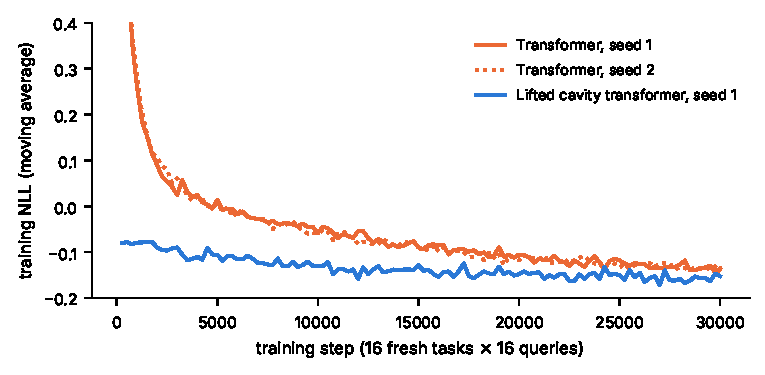
\includegraphics[width=.72\linewidth]{figures/training.pdf}
\caption{\label{fig:training}Training NLL (moving average; fresh tasks with at most one missing sensor) of the
transformer and the lifted cavity transformer, which share backbone, recipe and seed. The lifted output layer starts
at its anchor's closed form, so it begins far lower; the plain transformer must first learn fusion from scratch.}
\end{figure}

\section{Baselines and references}
\label{app:baselines}

\paragraph{Support-only closed forms.}
\begin{itemize}
  \item \textbf{EM-Gaussian:} the conditional of $y$ given $x_S$ under the EM joint Gaussian (40 iterations).
  \item \textbf{FA-Gaussian:} the closed form of \S\ref{sec:method}, with EM run for 40 iterations. The networks'
  anchors use 8 iterations and no variance inflation, so the reported FA-Gaussian is a slightly stronger baseline than
  the untrained networks (on F1 with two missing sensors, \FfaOnekc{} against \Untrainedkc).
  \item \textbf{NL-FA:} per-sensor cubic response curves in the standardized target. The intercept and slope are
  unpenalized; the curvature terms are ridge-penalized ($\lambda=100$) and clamped to the support's target range for
  linear extrapolation. The residual covariance has a one-factor structure. Exact inference is done on a 401-point
  grid. The degree and $\lambda$ were tuned on the development panel only: free degree selection by leave-one-out
  produced catastrophic extrapolation.
  \item \textbf{BLR:} evidence-maximized Bayesian linear regression~\citep{mackay1992bayesian} on complete-case
  rows, with predictive variance including parameter uncertainty.
  \item \textbf{Ridge:} complete-case ridge with leave-one-out residual variance, and the original mean-imputed ridge.
  \item \textbf{Gaussian process (post hoc):} for each episode and observed-sensor set, an ARD squared-exponential
  kernel plus white noise on the complete-case calibration rows, with hyperparameters by type-II maximum likelihood
  (one restart).
  \item \textbf{$k$-nearest neighbours (post hoc):} on the standardized observed sensors of complete-case calibration
  rows, with $k\in\{1,2,3,5,7,10\}$ chosen per episode and sensor set by leave-one-out NLL on the support and the
  leave-one-out mean squared error as predictive variance.
\end{itemize}
EM-Gaussian, FA-Gaussian and ridge inflate their predictive variance by $n/(n-|S|-1)$.

\paragraph{Bayes-optimal ceiling.}
The ceiling is HMC~\citep{neal2011hmc} over the 25 (or $5P$) task parameters. It uses the true priors, transformed to
unconstrained coordinates. The shared nuisance is marginalized analytically through a rank-one-plus-diagonal
covariance, using only the observed entries of each calibration row. The sign of each $a_j$ is fixed by the support
correlation, which is unambiguous because $|a_j|\geq0.6$.

The sampler runs 4 chains per task, each started from a MAP fit. Warm-up has two phases: step-size adaptation (target
acceptance $0.75$) and diagonal mass-matrix estimation from 150 iterations, followed by 150 more adaptation
iterations. We keep 50 draws per chain, thinned by 4, with 12 leapfrog steps.

The predictive density of a query uses the samples exactly, including the query's own reweighting:
$p(y\mid x_S,\D)=\sum_m p(y,x_S\mid\theta_m)/\sum_m p(x_S\mid\theta_m)$, with $p(x_S\mid\theta_m)$ by trapezoid
quadrature on 301 points. On every panel where it was run, R-hat on identifiable parameters was below 1.1 for at
least 99.9\% of parameters. Run with the true parameters, the predictive formula reproduces the exact oracle to
within $2\times10^{-3}$ nats (a unit test).

\section{Protocols and audit trail}
\label{app:audit}
\paragraph{How the method arose.}
The lifted cavity network replaced an earlier design that failed. That design was a three-round EP-style network whose
sites live on $y$ alone and are updated from the scalar cavity of $y$. It was evaluated under pre-registered gates on
the same synthetic family. Its first version collapsed to the prior during training. A repaired version, with sites
initialized from support moments, trained successfully but was beaten by a ridge regression. On that panel the
oracle, the ridge control and the best repaired seed scored:

\begin{center}\small
\begin{tabular}{lr}
\toprule
Method & NLL, two sensors missing\\
\midrule
Oracle & $-0.046$\\
Ridge control & $0.396$\\
Repaired scalar-cavity network (best seed) & $0.403$\\
\bottomrule
\end{tabular}
\end{center}

Computing the oracle exposed three problems. First, the control was weak: it mean-imputed missing calibration
entries, and a support-only EM or factor-analysis Gaussian scores 0.168 or 0.156. Second, scalar sites are
structurally limited (\S\ref{sec:scalar}). Third, the learners were starved: 512 reused tasks and 3{,}000 updates.
Retraining the scalar-cavity architecture with our recipe (60{,}000 tasks, 20{,}000 steps) improves it by only about
0.05 nats, and on F1 it remains \Ablrepocavityfreshvsfaabs\ nats worse than the untrained FA-Gaussian (\S\ref{sec:audit}).

\paragraph{Protocol v1.}
After development on panels that are now retired, five endpoints were committed to version control before their
panels were generated:
\begin{itemize}
  \item fresh synthetic tasks, against FA-Gaussian and against the residual MLP;
  \item 8-sensor transfer;
  \item stronger nonlinearity;
  \item a new real target (NO$_2$ on the Air Quality device).
\end{itemize}
All five passed (Table~\ref{tab:v1}). Each endpoint was evaluated once, and no model was retrained after the commit.

\begin{table}[h]
\centering\small
\caption{\label{tab:v1}Protocol v1 endpoints (two missing sensors; positive gain favours the lifted cavity network; pass requires gain $\geq0.01$ and a positive lower bound).}
\begin{tabular}{llcc}
\toprule
Endpoint & Comparison & Gain [95\% CI] & Result\\
\midrule
E1 & Fresh tasks, vs FA-Gaussian & $+$0.074 [$+$0.064, $+$0.084] & pass\\
E2 & Fresh tasks, vs residual MLP & $+$0.016 [$+$0.012, $+$0.020] & pass\\
E3 & 8 sensors, vs FA-Gaussian & $+$0.115 [$+$0.097, $+$0.132] & pass\\
E4 & Nonlinearity 0.8, vs residual MLP & $+$0.028 [$+$0.020, $+$0.036] & pass\\
R1 & Air Quality NO$_2$, 23 later weeks, vs EM-Gaussian & $+$0.112 [$+$0.050, $+$0.173] & pass\\
\bottomrule
\end{tabular}
\end{table}


\paragraph{Protocol v2.}
Protocol v2 was likewise committed before any of its panels or test splits existed. It adds:
\begin{itemize}
  \item the transformer baseline, NL-FA, BLR and the sign-conditioned HMC reference;
  \item wider panels (8 and 16 sensors), and shifts in nonlinearity and support size;
  \item the Beijing benchmark, whose test period had never been scored.
\end{itemize}
NL-FA's settings and BLR's choice as the strongest real-data closed form were fixed on development data
(Appendix~\ref{app:baselines}). The gas-sensor-drift dataset~\citep{vergara2012drift} was examined during development
and then excluded, before any test split was built. Its heavy-tailed sensor outliers made the mean NLL of every
Gaussian method dominated by a few episodes, with mean and median differing by more than 100 nats, so it cannot
separate methods. One deviation was recorded before any Beijing score existed: some query hours have no other station
observed, and complete-case BLR cannot fit zero features, so for an empty sensor set it returns the support mean with
variance $s^2(1+1/n)$, like the other closed forms' prior predictive.

\paragraph{Protocol v3.}
After protocol v2's real-data endpoint failed, protocol v3 was committed before any of its panels or targets existed.
It fixes one model (the lifted cavity transformer of \S\ref{sec:exp-v3}, trained once with the transformer's recipe
and seed and evaluated at its final checkpoint), two new synthetic panels (G1, G3), two Beijing pollutants never
scored by any model (NO$_2$, primary; CO, descriptive), the fine-tuning recipe of protocol v2, and four endpoints
(Table~\ref{tab:endpoints}). The lifted cavity transformer's scores on the v2 panels are descriptive only
(Appendix~\ref{app:more}). Two container restarts interrupted its training before any v3 score existed; it was retrained
from scratch with the same seed, and later runs checkpoint every random state so that a resumed run is bitwise
identical to an uninterrupted one (a unit test). The protocol document logs both events.

\paragraph{Post-hoc analyses.} Everything not named in a protocol is post hoc and labeled as such: the per-episode
Gaussian process and $k$-nearest neighbours, the second training seeds of both transformers, the fine-tuning diagnostics of \S\ref{sec:exp-real}, and the exploratory runs of
Appendix~\ref{app:more}.


\section{Broader impact}
\label{app:impact}
Calibrating low-cost environmental sensors widens access to air-quality monitoring. Overconfident predictions could
mislead exposure decisions, which is why we report coverage alongside likelihood. We recommend validating calibration
on each new deployment before relying on predicted intervals.

\section{Additional results}
\label{app:more}
\begin{table}[t]
\centering\small
\caption{\label{tab:ablation}Ablations on F1 (mean test NLL). Same training recipe for every learned row.}
\begin{tabular}{lcccc}
\toprule
Variant & $k{=}0$ & $k{=}1$ & $k{=}2$ & $k{=}3$\\
\midrule
Lifted cavity, $K=1$ (ours) & $-$0.265 & $-$0.112 & 0.097 & 0.395\\
Lifted cavity, $K=2$ & $-$0.267 & $-$0.112 & 0.098 & 0.397\\
Lifted sites, no cavity input & $-$0.221 & $-$0.074 & 0.123 & 0.399\\
Scalar sites ($K=0$), same machinery & $-$0.070 & 0.061 & 0.232 & 0.473\\
Scalar-cavity network (retrained) & 0.055 & 0.178 & 0.336 & 0.555\\
FA-Gaussian (untrained) & $-$0.152 & $-$0.011 & 0.177 & 0.439\\
\bottomrule
\end{tabular}
\end{table}

\begin{table}[t]
\centering\small
\caption{\label{tab:calib}Calibration and point accuracy. Coverage of the central 90\% predictive interval (target 0.90), continuous ranked probability score (CRPS, lower is better) and RMSE. F1 with two missing sensors; Beijing test with natural missingness (fine-tuned learned models).}
\begin{tabular}{lcccccc}
\toprule
 & \multicolumn{3}{c}{F1, $k=2$} & \multicolumn{3}{c}{Beijing, natural}\\
Method & Cov.\ 90 & CRPS & RMSE & Cov.\ 90 & CRPS & RMSE\\
\midrule
FA-Gaussian & 0.873 & 0.168 & 0.316 & 0.824 & 0.189 & 0.379\\
EM-Gaussian & 0.860 & 0.170 & 0.318 & 0.807 & 0.207 & 0.423\\
BLR & 0.866 & 0.174 & 0.327 & 0.861 & 0.182 & 0.374\\
Lifted cavity (ours) & 0.901 & 0.160 & 0.305 & 0.914 & 0.171 & 0.357\\
Transformer & 0.902 & 0.165 & 0.314 & 0.914 & 0.158 & 0.341\\
Residual MLP & 0.902 & 0.162 & 0.309 & -- & -- & --\\
\bottomrule
\end{tabular}
\end{table}

\begin{table}[h]
\centering\small
\caption{\label{tab:explore}Post-hoc fine-tuning variants on Beijing PM$_{2.5}$ (test period of protocol v2; mean test NLL). Neither more nuisance dimensions nor longer fine-tuning closes the gap to the fine-tuned transformer.}
\begin{tabular}{lccc}
\toprule
Fine-tuned model & natural & $+3$ & $+6$\\
\midrule
Lifted cavity network, standard recipe (seed 1) & 0.207 & 0.237 & 0.304\\
\quad with $K=2$ & 0.205 & 0.239 & 0.300\\
\quad with $5\times$ fine-tuning steps & 0.169 & 0.201 & 0.276\\
Transformer, standard recipe & 0.087 & 0.121 & 0.236\\
\bottomrule
\end{tabular}
\end{table}

\begin{table}[h]
\centering\small
\caption{\label{tab:moreF2}Panel F2 (8 sensors; 128 tasks): mean test NLL by number of missing sensors.}
\begin{tabular}{lcccc}
\toprule
Method & $k{=}0$ & $k{=}1$ & $k{=}2$ & $k{=}3$\\
\midrule
Oracle & $-$0.807 & $-$0.712 & $-$0.598 & $-$0.459\\
FA-Gaussian & $-$0.462 & $-$0.387 & $-$0.296 & $-$0.183\\
EM-Gaussian & 0.032 & $-$0.133 & $-$0.160 & $-$0.120\\
NL-FA & $-$0.485 & $-$0.414 & $-$0.327 & $-$0.215\\
BLR & 0.187 & 0.398 & 0.615 & 0.028\\
Ridge (complete case) & 0.064 & $-$0.003 & $-$0.033 & $-$0.015\\
Lifted cavity (ours) & $-$0.615 & $-$0.530 & $-$0.427 & $-$0.302\\
Lifted cavity, $K=2$ & $-$0.618 & $-$0.531 & $-$0.427 & $-$0.302\\
Lifted sites, no cavity & $-$0.551 & $-$0.469 & $-$0.369 & $-$0.250\\
Scalar sites ($K=0$) & $-$0.295 & $-$0.228 & $-$0.148 & $-$0.057\\
Transformer & $-$0.568 & $-$0.474 & $-$0.362 & $-$0.229\\
Transformer, all masks & $-$0.545 & $-$0.452 & $-$0.343 & $-$0.212\\
Lifted cavity transformer (v3) & $-$0.611 & $-$0.526 & $-$0.423 & $-$0.299\\
\bottomrule
\end{tabular}
\end{table}

\begin{table}[h]
\centering\small
\caption{\label{tab:moreF3}Panel F3 (16 sensors; 128 tasks): mean test NLL by number of missing sensors.}
\begin{tabular}{lcccc}
\toprule
Method & $k{=}0$ & $k{=}1$ & $k{=}2$ & $k{=}3$\\
\midrule
Oracle & $-$1.223 & $-$1.184 & $-$1.142 & $-$1.096\\
FA-Gaussian & $-$0.864 & $-$0.832 & $-$0.797 & $-$0.758\\
EM-Gaussian & 6.300 & 4.851 & 2.977 & 1.553\\
NL-FA & $-$0.910 & $-$0.876 & $-$0.841 & $-$0.803\\
BLR & 0.095 & 0.078 & 0.058 & 0.054\\
Ridge (complete case) & 0.093 & 0.089 & 0.081 & 0.086\\
Lifted cavity (ours) & $-$1.018 & $-$0.982 & $-$0.945 & $-$0.902\\
Lifted cavity, $K=2$ & $-$1.017 & $-$0.981 & $-$0.944 & $-$0.901\\
Lifted sites, no cavity & $-$0.952 & $-$0.916 & $-$0.880 & $-$0.836\\
Scalar sites ($K=0$) & $-$0.658 & $-$0.627 & $-$0.591 & $-$0.554\\
Transformer & $-$0.886 & $-$0.846 & $-$0.801 & $-$0.747\\
Transformer, all masks & $-$0.869 & $-$0.832 & $-$0.790 & $-$0.738\\
Lifted cavity transformer (v3) & $-$1.020 & $-$0.985 & $-$0.949 & $-$0.905\\
\bottomrule
\end{tabular}
\end{table}

\begin{table}[h]
\centering\small
\caption{\label{tab:moreF4}Panel F4 (nonlinearity 0.8; 128 tasks): mean test NLL by number of missing sensors.}
\begin{tabular}{lcccc}
\toprule
Method & $k{=}0$ & $k{=}1$ & $k{=}2$ & $k{=}3$\\
\midrule
Oracle & $-$0.513 & $-$0.331 & $-$0.086 & 0.261\\
FA-Gaussian & 0.050 & 0.170 & 0.334 & 0.568\\
EM-Gaussian & 0.050 & 0.145 & 0.311 & 0.559\\
NL-FA & $-$0.032 & 0.089 & 0.258 & 0.507\\
BLR & 0.208 & 0.188 & 0.331 & 0.568\\
Ridge (complete case) & 0.138 & 0.208 & 0.338 & 0.571\\
Lifted cavity (ours) & $-$0.185 & $-$0.026 & 0.191 & 0.498\\
Lifted cavity, $K=2$ & $-$0.200 & $-$0.035 & 0.186 & 0.497\\
Lifted sites, no cavity & $-$0.068 & 0.075 & 0.261 & 0.519\\
Scalar sites ($K=0$) & $-$0.013 & 0.130 & 0.314 & 0.570\\
Transformer & $-$0.226 & $-$0.043 & 0.191 & 0.503\\
Transformer, all masks & $-$0.221 & $-$0.038 & 0.190 & 0.486\\
Residual MLP & $-$0.107 & 0.039 & 0.235 & 0.508\\
Scalar-cavity network & 0.133 & 0.256 & 0.416 & 0.635\\
Lifted cavity transformer (v3) & $-$0.196 & $-$0.037 & 0.179 & 0.482\\
\bottomrule
\end{tabular}
\end{table}

\begin{table}[h]
\centering\small
\caption{\label{tab:moreF5}Panel F5 (linear sensors; 128 tasks): mean test NLL by number of missing sensors.}
\begin{tabular}{lcccc}
\toprule
Method & $k{=}0$ & $k{=}1$ & $k{=}2$ & $k{=}3$\\
\midrule
Oracle & $-$0.455 & $-$0.288 & $-$0.066 & 0.244\\
FA-Gaussian & $-$0.362 & $-$0.203 & 0.009 & 0.305\\
EM-Gaussian & $-$0.244 & $-$0.142 & 0.034 & 0.308\\
NL-FA & $-$0.337 & $-$0.178 & 0.030 & 0.318\\
BLR & $-$0.135 & $-$0.085 & 0.061 & 0.322\\
Ridge (complete case) & $-$0.169 & $-$0.092 & 0.062 & 0.323\\
Lifted cavity (ours) & $-$0.323 & $-$0.172 & 0.031 & 0.318\\
Lifted cavity, $K=2$ & $-$0.320 & $-$0.170 & 0.033 & 0.318\\
Lifted sites, no cavity & $-$0.343 & $-$0.189 & 0.018 & 0.309\\
Scalar sites ($K=0$) & $-$0.085 & 0.031 & 0.186 & 0.415\\
Transformer & $-$0.278 & $-$0.122 & 0.085 & 0.371\\
Transformer, all masks & $-$0.281 & $-$0.123 & 0.080 & 0.353\\
Residual MLP & $-$0.304 & $-$0.161 & 0.036 & 0.319\\
Scalar-cavity network & 0.052 & 0.161 & 0.302 & 0.505\\
Lifted cavity transformer (v3) & $-$0.319 & $-$0.171 & 0.029 & 0.315\\
\bottomrule
\end{tabular}
\end{table}

\begin{table}[h]
\centering\small
\caption{\label{tab:moreF6}Panel F6 (16 support rows; 128 tasks): mean test NLL by number of missing sensors.}
\begin{tabular}{lcccc}
\toprule
Method & $k{=}0$ & $k{=}1$ & $k{=}2$ & $k{=}3$\\
\midrule
Oracle & $-$0.446 & $-$0.280 & $-$0.060 & 0.252\\
FA-Gaussian & 0.256 & 0.371 & 0.510 & 0.686\\
EM-Gaussian & 24.900 & 4.682 & 1.140 & 0.739\\
NL-FA & 0.314 & 0.388 & 0.496 & 0.661\\
BLR & 0.898 & 0.857 & 3.690 & 0.887\\
Ridge (complete case) & 0.317 & 0.391 & 0.500 & 0.624\\
Lifted cavity (ours) & 0.073 & 0.195 & 0.363 & 0.604\\
Lifted cavity, $K=2$ & 0.156 & 0.250 & 0.392 & 0.614\\
Lifted sites, no cavity & 0.117 & 0.234 & 0.389 & 0.604\\
Scalar sites ($K=0$) & 0.204 & 0.293 & 0.428 & 0.644\\
Transformer & 0.253 & 0.371 & 0.523 & 0.731\\
Transformer, all masks & 0.256 & 0.359 & 0.483 & 0.653\\
Residual MLP & 0.094 & 0.211 & 0.371 & 0.594\\
Scalar-cavity network & 0.345 & 0.439 & 0.565 & 0.750\\
Lifted cavity transformer (v3) & 0.237 & 0.333 & 0.457 & 0.643\\
\bottomrule
\end{tabular}
\end{table}

\begin{table}[h]
\centering\small
\caption{\label{tab:moreF7}Panel F7 (96 support rows; 128 tasks): mean test NLL by number of missing sensors.}
\begin{tabular}{lcccc}
\toprule
Method & $k{=}0$ & $k{=}1$ & $k{=}2$ & $k{=}3$\\
\midrule
Oracle & $-$0.429 & $-$0.264 & $-$0.043 & 0.269\\
FA-Gaussian & $-$0.232 & $-$0.082 & 0.114 & 0.385\\
EM-Gaussian & $-$0.237 & $-$0.086 & 0.112 & 0.385\\
NL-FA & $-$0.276 & $-$0.127 & 0.073 & 0.353\\
BLR & $-$0.178 & $-$0.056 & 0.125 & 0.390\\
Ridge (complete case) & $-$0.163 & $-$0.047 & 0.129 & 0.391\\
Lifted cavity (ours) & $-$0.324 & $-$0.163 & 0.052 & 0.353\\
Lifted cavity, $K=2$ & $-$0.320 & $-$0.159 & 0.056 & 0.357\\
Lifted sites, no cavity & $-$0.275 & $-$0.123 & 0.078 & 0.359\\
Scalar sites ($K=0$) & $-$0.097 & 0.034 & 0.205 & 0.443\\
Transformer & $-$0.295 & $-$0.133 & 0.081 & 0.379\\
Transformer, all masks & $-$0.297 & $-$0.134 & 0.080 & 0.367\\
Residual MLP & $-$0.287 & $-$0.131 & 0.074 & 0.360\\
Scalar-cavity network & 0.047 & 0.161 & 0.309 & 0.516\\
Lifted cavity transformer (v3) & $-$0.329 & $-$0.167 & 0.047 & 0.346\\
\bottomrule
\end{tabular}
\end{table}

\begin{table}[h]
\centering\small
\caption{\label{tab:moreairqco}Air Quality CO: mean test NLL for every number of simulated missing sensors (23 later weeks).}
\begin{tabular}{lcccc}
\toprule
Method & $k{=}0$ & $k{=}1$ & $k{=}2$ & $k{=}3$\\
\midrule
EM-Gaussian & 0.074 & 0.063 & 0.085 & 0.146\\
FA-Gaussian & 0.052 & 0.086 & 0.116 & 0.154\\
NL-FA & 0.144 & 0.120 & 0.091 & 0.124\\
Bayesian linear regression & 1.037 & 0.433 & 0.216 & 0.202\\
Ridge (complete case) & 0.824 & 0.337 & 0.208 & 0.210\\
GP, complete case$^\dagger$ & 3.364 & 1.056 & 0.503 & 0.146\\
$k$-nearest neighbours$^\dagger$ & 0.571 & 0.391 & 0.353 & 0.274\\
Lifted cavity, zero-shot & 0.044 & 0.064 & 0.129 & 0.160\\
Transformer, zero-shot & $-$0.017 & $-$0.006 & 0.081 & 0.154\\
\textbf{Lifted cavity, fine-tuned (ours)} & $-$0.040 & $-$0.031 & 0.008 & 0.077\\
\quad no synthetic pretraining & $-$0.001 & $-$0.014 & $-$0.006 & 0.077\\
\quad no cavity input & $-$0.086 & $-$0.065 & $-$0.028 & 0.038\\
\quad scalar sites ($K=0$) & $-$0.026 & $-$0.021 & $-$0.003 & 0.075\\
Transformer, fine-tuned & $-$0.163 & $-$0.149 & $-$0.052 & 0.036\\
Residual MLP, fine-tuned & 0.025 & 0.061 & 0.110 & 0.160\\
\bottomrule
\end{tabular}
\end{table}

\begin{table}[h]
\centering\small
\caption{\label{tab:moreairqno2}Air Quality NO$_2$: mean test NLL for every number of simulated missing sensors (23 later weeks).}
\begin{tabular}{lcccc}
\toprule
Method & $k{=}0$ & $k{=}1$ & $k{=}2$ & $k{=}3$\\
\midrule
EM-Gaussian & $-$0.237 & $-$0.174 & $-$0.175 & $-$0.168\\
FA-Gaussian & $-$0.196 & $-$0.173 & $-$0.155 & $-$0.162\\
NL-FA & $-$0.090 & $-$0.102 & $-$0.142 & $-$0.169\\
Bayesian linear regression & $-$0.055 & $-$0.214 & $-$0.178 & $-$0.160\\
Ridge (complete case) & $-$0.200 & $-$0.230 & $-$0.176 & $-$0.145\\
GP, complete case$^\dagger$ & 25.217 & 0.696 & $-$0.198 & $-$0.258\\
$k$-nearest neighbours$^\dagger$ & $-$0.010 & $-$0.020 & $-$0.063 & $-$0.128\\
Lifted cavity, zero-shot & $-$0.350 & $-$0.295 & $-$0.233 & $-$0.176\\
Transformer, zero-shot & $-$0.360 & $-$0.310 & $-$0.231 & $-$0.136\\
\textbf{Lifted cavity, fine-tuned (ours)} & $-$0.412 & $-$0.366 & $-$0.337 & $-$0.273\\
\quad no synthetic pretraining & $-$0.419 & $-$0.365 & $-$0.316 & $-$0.248\\
\quad no cavity input & $-$0.423 & $-$0.375 & $-$0.332 & $-$0.275\\
\quad scalar sites ($K=0$) & $-$0.359 & $-$0.337 & $-$0.302 & $-$0.231\\
Transformer, fine-tuned & $-$0.485 & $-$0.429 & $-$0.381 & $-$0.294\\
Residual MLP, fine-tuned & $-$0.246 & $-$0.198 & $-$0.147 & $-$0.106\\
\bottomrule
\end{tabular}
\end{table}

